\documentclass[11pt]{article}

\usepackage[margin=1.05in]{geometry}
\usepackage[T1]{fontenc}
\usepackage[utf8]{inputenc}
\usepackage{lmodern}
\usepackage{microtype}
\usepackage{amsmath,amssymb,amsthm,mathtools}
\usepackage{enumitem}
\usepackage{booktabs}
\usepackage{xcolor}
\usepackage{tikz}
\usepackage{tikz-cd}
\usetikzlibrary{arrows.meta,calc,positioning,decorations.pathreplacing,fit,backgrounds}
\usepackage{hyperref}
\usepackage[nameinlink,capitalize,noabbrev]{cleveref}
\usepackage[backend=biber,style=alphabetic,maxnames=6]{biblatex}
\addbibresource{kato_collapse_refs.bib}

\hypersetup{
  colorlinks=true,
  linkcolor=blue!50!black,
  citecolor=blue!50!black,
  urlcolor=blue!55!black,
  pdftitle={Collapse-depth towers, Kato fans, and adic topology},
  pdfauthor={Tyler Foster and ChatGPT}
}

\newtheorem{question}{Question}
\newtheorem{principle}{Principle}
\newtheorem{warning}{Warning}
\newtheorem{claim}{Claim}
\newtheorem{definition}{Definition}
\newtheorem{example}{Example}
\newtheorem{remark}{Remark}

\newcommand{\A}{\mathbb A}
\newcommand{\Z}{\mathbb Z}
\newcommand{\N}{\mathbb N}
\newcommand{\R}{\mathbb R}
\newcommand{\C}{\mathbb C}
\newcommand{\Q}{\mathbb Q}
\newcommand{\Spec}{\operatorname{Spec}}
\newcommand{\Spf}{\operatorname{Spf}}
\newcommand{\Spa}{\operatorname{Spa}}
\newcommand{\Hom}{\operatorname{Hom}}
\newcommand{\colim}{\operatorname{colim}}
\newcommand{\red}{\operatorname{red}}
\newcommand{\val}{\mathrm{val}}
\newcommand{\ad}{\mathrm{ad}}
\newcommand{\an}{\mathrm{an}}
\newcommand{\tor}{\mathrm{tor}}
\newcommand{\bA}{\mathbf A}
\newcommand{\mfX}{\mathfrak X}
\newcommand{\mfY}{\mathfrak Y}
\newcommand{\fs}{\mathrm{fs}}

\title{Collapse-depth towers, Kato fans, and adic topology\\
\large Notes extracting the mathematical content of a conversation}
\author{Prepared for Tyler Foster\\
\small with explicit attribution of the central viewpoint to Tyler Foster}
\date{June 2026}

\begin{document}
\maketitle

\begin{abstract}
These notes record and reorganize a conversation about toroidal degenerations, Kato fans, inverse systems of collapses, and their relation to adic topology. The central mathematical viewpoint was supplied by Tyler Foster. The assistant initially kept returning to standard facts about node thickness, tropical edge length, valuativization, and skeleta. Tyler's point was sharper: a visible horizontal collapse in a fixed degeneration should be read as a shadow of vertical movement in a system of lower and higher models, and the serious theorem is a duality/cofinality statement explaining when and how such horizontal collapse data is realized by actual model maps. The familiar global object behind the inverse system of all such Kato-fan subdivisions and collapses is Kato's valuativization, or the logarithmic/combinatorial Riemann--Zariski space; in analytic language its rank-one real shadow is a skeleton inside a Berkovich or adic generic fiber.
\end{abstract}

\tableofcontents

\section{Attribution and purpose}

This document is deliberately written with strong attribution. The conceptual thread was not supplied by the assistant. Tyler Foster supplied the key research question and repeatedly corrected weaker answers that stopped at standard material.

The assistant first described familiar facts:
\begin{itemize}[leftmargin=2em]
\item local nodes of thickness $n$ have equation $xy=t^n$;
\item tropical edge lengths are valuations of smoothing parameters;
\item Kato fans and cone complexes organize toroidal/logarithmic strata;
\item the inverse system over all log blowups is Kato valuativization;
\item Berkovich and Huber analytic spaces contain skeletal loci.
\end{itemize}
These statements were not the point. Tyler's question was about the missing bridge between a \emph{horizontal collapse visible in one degeneration} and a \emph{vertical transition in a system of models}. More precisely, Tyler asked whether one can read from a fixed higher model $\mfY$ that there exists a lower model $\mfX$ such that the visible horizontal chain in $\mfY_s$ collapses under a morphism $\mfY\to\mfX$. That is the part that had to be forced into focus.

The point of these notes is to isolate that question and put it in language useful for researchers.

\section{The starting toy model: two different node thicknesses}

Let the base be the toric affine line
\[
S=\Spec k[t]
\]
with its standard log structure. A nodal degeneration whose special fiber has three components in a chain
\[
C_0 - C_1 - C_2
\]
can have different smoothing orders at the two nodes. Locally one may have
\[
q_{01}:\quad xy=t^2,
\qquad
q_{12}:\quad uv=t.
\]
Thus the weighted dual graph is
\[
\ast \xleftrightarrow{\;2\;} \ast \xleftrightarrow{\;1\;} \ast.
\]
The integer $n$ in $xy=t^n$ is the thickness of the node, or equivalently the length of the corresponding edge in the tropical curve when $v(t)=1$. This is standard in the stable-reduction and tropical-curve dictionary.

A toric fan presentation of the same local phenomenon is obtained as follows. Let
\[
N_X=\Z^2,
\qquad
N_B=\Z,
\qquad
h(a,b)=b.
\]
The base fan is the fan of $\A^1$, namely $\{0,\R_{\ge 0}\}$. In $N_X$ take height-one rays
\[
v_0=(0,1),\qquad v_1=(2,1),\qquad v_2=(3,1),
\]
and the two cones
\[
\sigma_{01}=\langle v_0,v_1\rangle,
\qquad
\sigma_{12}=\langle v_1,v_2\rangle.
\]
The determinants are $2$ and $1$, respectively. The corresponding local toric charts are
\[
xy=t^2,
\qquad
uv=t.
\]
The total space is normal at $xy=t^2$; it is singular but not non-normal.

\begin{figure}[h]
\centering
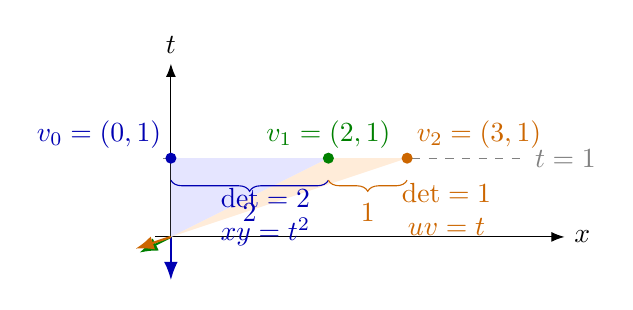
\begin{tikzpicture}[scale=1.0,>=Latex]
  \draw[->] (-0.2,0) -- (5.0,0) node[right] {$x$};
  \draw[->] (0,-0.2) -- (0,2.2) node[above] {$t$};
  \draw[dashed,gray] (-0.1,1) -- (4.5,1) node[right] {$t=1$};
  \coordinate (O) at (0,0);
  \coordinate (v0) at (0,1);
  \coordinate (v1) at (2,1);
  \coordinate (v2) at (3,1);
  \fill[blue!10] (O)--(v0)--(v1)--cycle;
  \fill[orange!15] (O)--(v1)--(v2)--cycle;
  \draw[blue!70!black,thick,->] (O)--($(v0)!1.55!(O)$);
  \draw[green!50!black,thick,->] (O)--($(v1)!1.20!(O)$);
  \draw[orange!80!black,thick,->] (O)--($(v2)!1.15!(O)$);
  \fill[blue!70!black] (v0) circle (2pt) node[above left] {$v_0=(0,1)$};
  \fill[green!50!black] (v1) circle (2pt) node[above] {$v_1=(2,1)$};
  \fill[orange!80!black] (v2) circle (2pt) node[above right] {$v_2=(3,1)$};
  \draw[decorate,decoration={brace,mirror,amplitude=4pt},blue!70!black] (0,0.72)--(2,0.72) node[midway,below=5pt] {$2$};
  \draw[decorate,decoration={brace,mirror,amplitude=4pt},orange!80!black] (2,0.72)--(3,0.72) node[midway,below=5pt] {$1$};
  \node[blue!70!black,align=center] at (1.2,0.25) {$\det=2$\\$xy=t^2$};
  \node[orange!80!black,align=center] at (3.5,0.35) {$\det=1$\\$uv=t$};
\end{tikzpicture}
\caption{The toric fan fragment over the base ray. The height-one slice has lattice gaps $2$ and $1$.}
\label{fig:fan}
\end{figure}

\section{What the standard answer says, and why it was not enough}

The standard tropical statement is:
\[
xy=t^n \quad\leadsto\quad \ell(e)=n.
\]
Equivalently, if a nodal smoothing parameter is $q_e=t^n$, then the tropical edge length is $v(q_e)=n$.
This is useful, but it was not Tyler's question.

Tyler's point was that interpreting $n$ as a metric length is still the familiar tropical move. A more adic/profinite interpretation is to treat $n$ as a \emph{depth in an inverse system}. The toy chain
\[
\{[0],[1],[2]\}
\longrightarrow
\{[0,1],[2]\}
\longrightarrow
\{[0,1,2]\}
\]
should not be viewed merely as a metric graph with edge lengths. It is a finite quotient tower: points or components are indistinguishable to one level, then to a deeper level, then entirely collapsed at a still coarser level.

The analogy Tyler insisted on is the elementary one
\[
\Z_p \simeq \varprojlim_n \Z/p^n\Z.
\]
The topology on $\Z_p$ is not obtained by first drawing a metric tree; it is the inverse-limit topology of finite congruence quotients. Tyler's question was whether the edge-depth data in toroidal/log degenerations is a manifestation of this same kind of inverse-system topology.

\section{The corrected problem: horizontal collapse versus vertical model maps}

The decisive correction was the following. The chain
\[
[0]--[1]--[2]
\longrightarrow
[0,1]--[2]
\longrightarrow
[0,1,2]
\]
looks horizontal if one stares only at a special fiber or a dual graph. But in the geometry of models it should arise from vertical arrows
\[
\mfY_2\longrightarrow \mfY_1\longrightarrow \mfY_0
\]
in a category of models. Applying a shadow functor -- special-fiber strata, Kato fan, cone complex, or reduction partition -- produces the displayed horizontal-looking collapse.

The subtle part is not that a vertical map of models induces a map on shadows. That is formal. The hard part is the converse/existence problem:

\begin{question}[Tyler Foster's formulation]
Given a fixed higher toroidal or logarithmic model $\mfY$, can one read in the horizontal degeneration data of $\mfY_s$ that $\mfY$ lies above a lower model $\mfX$? Equivalently, when does a visible horizontal collapse of strata/components extend to an actual morphism of models
\[
\mfY\longrightarrow \mfX?
\]
\end{question}

This is the point at which the conversation finally reached the real question. The graph is not the theorem. The theorem, if true in a given setting, says that the desired horizontal collapse data can be lifted to, or detected as, a vertical relation among models.

\section{Reading a lower model from a fixed higher model}

Let $\mfY$ be a toroidal/log model, with Kato fan or cone complex
\[
F_{\mfY}\longrightarrow F_S.
\]
A lower model $\mfX$ corresponds, combinatorially, to a coarser Kato fan or cone complex $F_{\mfX}$ together with a subdivision map
\[
F_{\mfY}\longrightarrow F_{\mfX}.
\]
Geometrically this is the shadow of a log blowup, toroidal modification, or model domination map
\[
\mfY\longrightarrow \mfX.
\]
Thus the internal test is:
\[
\boxed{
\text{Does the proposed horizontal collapse extend to a coarser Kato fan/cone complex?}
}
\]
If yes, then the horizontal chain is not merely a heuristic drawing; it records the existence of a lower model.

In the fan of \cref{fig:fan}, the two-cone fan with rays $v_0,v_1,v_2$ is a subdivision of the one-cone fan with rays $v_0,v_2$. Removing the interior wall is a coarsening of the fan. In this case the higher model is visibly a toric modification of a lower model. The horizontal chain in the special fiber is a witness for a vertical blowdown.

\begin{figure}[h]
\centering
\begin{tikzcd}[column sep=large,row sep=large]
\mfY \arrow[d] \arrow[r,mapsto] & \{[0],[1],[2]\} \arrow[d] \\
\mfX_1 \arrow[d] \arrow[r,mapsto] & \{[0,1],[2]\} \arrow[d] \\
\mfX_0 \arrow[r,mapsto] & \{[0,1,2]\}
\end{tikzcd}
\caption{The issue Tyler isolated: horizontal collapse data should be realized by vertical model maps. The existence of the left-hand vertical arrows with precisely the desired right-hand shadows is the substantive assertion.}
\label{fig:vertical-horizontal}
\end{figure}

\section{A functorial construction from one fixed model}

One way to package the finite collapse tower from a fixed degeneration is as follows. Suppose the base characteristic monoid is $\N$, with its ideal filtration
\[
I_r=r+\N\subset \N.
\]
For a curve-like toroidal degeneration, the local smoothing parameter of an edge $e$ gives an element
\[
\delta_e\in \N.
\]
From this one obtains a finite collapse tower
\[
Q_r(\mfY)=\pi_0(\Gamma_{\delta\ge r}),
\]
where $\Gamma_{\delta\ge r}$ is the subgraph consisting of edges whose smoothing depth lies in $I_r$, i.e. $\delta_e\ge r$. For the fan with edge depths $2$ and $1$ this gives
\[
Q_3=\{[0],[1],[2]\},
\]
\[
Q_2=\{[0,1],[2]\},
\]
\[
Q_1=\{[0,1,2]\}.
\]
This construction is the fixed-model, base-ideal collapse tower.

However, one must be careful. The quotients appearing in this tower need not be honest quotients in the category of ordinary saturated Kato fans. They may pass through stacky, torsion, non-saturated, or residue-decorated quotients if formulated too naively. Tyler's correction was that the relevant geometric category is not simply ``linear quotient of the ambient lattice fan.'' In actual models of $\A^1$ over a DVR, divisors and blowdowns can realize such quotient behavior geometrically even when the naive lattice quotient language is misleading.

Thus the safe formulation is not:
\[
\text{every collapse partition is an ordinary Kato-fan quotient.}
\]
It is:
\begin{center}
\fbox{\begin{minipage}{0.88\textwidth}
A fixed model produces a tower of finite reduction/collapse shadows, and the hard question is which such shadows are realized by lower models.
\end{minipage}}
\end{center}

\section{Relation to cofinality and adic topology}

The global version of the question asks what happens when one ranges not over one fixed $\mfY$, but over all suitable toroidal, logarithmic, or Gubler models. Foster--Payne prove a precise theorem in the toric/Gubler setting: adic tropicalizations are constructed as limits of Gubler models associated to polyhedral covers, and Huber analytification is recovered as an inverse limit of these adic tropicalizations; the key technical input is cofinality of Gubler models \cite{FosterPayneAdicTropicalizations,FosterIntroAdicTropicalization}.

This is the correct high-level analogue of the elementary identity
\[
\Z_p=\varprojlim_n \Z/p^n\Z.
\]
The finite quotients are not arbitrary graphs. They are model-level finite approximations. The topology is recovered because the model system is cofinal among the relevant adic approximations.

The chain
\[
\{[0],[1],[2]\}
\to
\{[0,1],[2]\}
\to
\{[0,1,2]\}
\]
is therefore best understood as a one-dimensional toy shadow of a cofinal inverse system. It is not the general theorem. In higher dimensions the graph must be replaced by polyhedral or cone-complex data, and in actual analytic geometry one must also account for residue-field or initial-degeneration information.

\section{Inverse systems of Kato-fan collapses and valuativization}

The familiar object associated to the massive inverse system over all log blowups/subdivisions of a Kato fan is Kato's valuativization. In log-geometric language, valuativization is obtained as an inverse limit over log blowups; Scherotzke--Sibilla--Talpo describe the valuativization as the projective limit of every possible log blowup \cite{ScherotzkeSibillaTalpo}. Illusie's survey of Kato's logarithmic spaces also describes the valuative construction in this inverse-limit spirit \cite{IllusieLogSpaces,KatoLogDieudonne}.

Combinatorially, log blowups correspond to subdivisions of Kato fans. Hence the inverse system of all refined Kato fans, with transition maps that collapse refinements back to coarser fans, is the Kato-fan side of valuativization.

One should distinguish:
\begin{enumerate}[leftmargin=2em]
\item the \emph{fixed-model collapse tower} extracted from one $F_{\mfY}\to F_S$;
\item the \emph{all-model inverse system} over log blowups/subdivisions;
\item the \emph{analytic or adic generic fiber}, which contains more points and more residue data than the combinatorial skeleton alone.
\end{enumerate}
The first was Tyler's central finite object. The second is the familiar valuativization. The third is the ambient analytic object whose topology is recovered, in suitable theorems, from a cofinal system of model-level approximations.

\section{Where this lives inside the Berkovich affine line}

For the Berkovich affine line $\A^{1,\an}_K$, a useful mental picture is a tree of closed disks. Type I points are classical points, which behave like leaves. Type II and III points form the visible disk/tree skeleton: type II points are disk points with radius in $|K^\ast|$, while type III points have radius outside $|K^\ast|$; type IV points are limiting endpoints of decreasing disks. This classification is standard in expositions of the Berkovich affine line \cite{BakerBerkovichNotes,PoineauTurchetti}.

The Kato-fan valuativization should not be identified with the whole Berkovich affine line. It is closer to the monomial/skeletal part: the tree part of the affine line with the classical residue-field leaves stripped away. In a rank-one real-valued picture, it is the type II/III disk skeleton. In a genuinely adic or valuative picture, it is better regarded as an all-ranks monomial or logarithmic Riemann--Zariski skeleton.

Thus the slogan is:
\[
\boxed{
\text{Kato fan }F \leadsto \text{finite skeleton};
\qquad
F^{\val} \leadsto \text{valuative/logarithmic skeleton}.
}
\]
The ordinary skeleton is a real-valued shadow. Valuativization remembers compatible centers through all subdivisions/log blowups and therefore behaves like the combinatorial Riemann--Zariski space of the toroidal/log structure.

\section{Final distilled formulation}

The whole conversation can be compressed into the following sequence.

\begin{enumerate}[leftmargin=2em]
\item A toroidal degeneration with local equations $xy=t^2$ and $uv=t$ gives a weighted chain of thicknesses $2$ and $1$.
\item The metric interpretation of these thicknesses is standard and was not Tyler's main question.
\item Tyler's point was to reinterpret thickness/collapse depth as inverse-system depth, analogous to congruence depth in $\Z_p=\varprojlim\Z/p^n\Z$.
\item The key finite object is a collapse tower extracted from one fixed model $\mfY$, such as
\[
\{[0],[1],[2]\}\to\{[0,1],[2]\}\to\{[0,1,2]\}.
\]
\item The hard geometric question is whether such a horizontal collapse tower is realized by vertical morphisms to lower models.
\item When it is realized, the horizontal collapse is read as a coarsening of the Kato fan/cone complex, hence as a blowdown or lower-model relation.
\item Ranging over all log blowups/subdivisions leads to Kato valuativization. This is the logarithmic or combinatorial Riemann--Zariski object.
\item In analytic geometry, the rank-one real-valued shadow is the usual skeleton inside a Berkovich or adic generic fiber. For $\A^1$ it is well pictured as the disk/tree part without the classical leaves.
\end{enumerate}

\section*{Acknowledgement of the mathematical contribution in the exchange}

The central formulation in these notes is Tyler Foster's. In particular, Tyler supplied the transition from:
\[
\text{edge length as tropical metric}
\]
to
\[
\text{edge/collapse depth as inverse-system data},
\]
and then to the sharper question:
\[
\text{can a horizontal collapse visible in one model be recognized as a vertical map to a lower model?}
\]
The assistant's earlier responses repeatedly answered weaker questions: node thickness, ordinary skeleta, full valuativization, and the existence of general model inverse limits. Tyler forced the distinction that the finite collapse tower from a fixed degeneration is the essential local object, while Kato valuativization and adic tropicalization provide the global/inverse-system context.

\nocite{UlirschFunctorialTropicalization,UlirschArtinFans,AbramovichCaporasoPayne,AbramovichChenMarcusUlirschWise,TalpoVistoliInfiniteRootStacks}
\printbibliography

\end{document}
